\documentclass[sigconf]{acmart}
\usepackage{multicol}
\usepackage{multirow}
\usepackage{graphicx}


\setcopyright{none}    % Disables ACM copyright notice
\acmConference{}{}{}   % Removes conference information
\acmBooktitle{}        % Removes book title
\acmDOI{}              % Removes DOI
\acmISBN{}             % Removes ISBN
\settopmatter{printacmref=false} % Removes the ACM reference format notice
\renewcommand\footnotetextcopyrightpermission[1]{}


\title{Midpoint Project Report: SQL Auto-Optimization Using Random Forests}
\author{Austin Mitchell}
\affiliation{%
  \institution{Georgia Institute of Technology}
  \city{Atlanta, GA}
  \country{United States}
}
\email{amitchell80@gatech.edu}

\graphicspath{{../../images/}}

\begin{document}

\maketitle

\section{Introduction}
The overall purpose of this project was to create a Machine Learning model, using Random Forest regressions, to predict the execution times of PostgreSQL
queries. This model could then be utilized in the training of another model in order to efficiently predict the execution time of a proposed version of a query
by an optimizer. This would allow an optimizer to compare between several possibilities without having to execute the query as a whole. This is supposed to be
utilized as an exploratory measure of how machine learning could be leveraged for applications in the database systems space.

\section{Updated Methodology}
Originally, when I created this project, I was going to utilize a feature set obtained from the \texttt{EXPLAIN ANALYZE} command in PostgreSQL, 
before moving on to the next steps of making an optimizer. This feature set would be used to then train a regression to predict the execution time 
of the proposed optimized queries. However, I realized that this might not be a completely predictable way for a prediction to take place as this requires
the query to be ran prior to the prediction, which doesn't make a lot of sense. I still created this regression just to evaluate its effectiveness, but I do
not think it would be wise to utilize this in the evaluation of proposed optimized models. So, in addition to the feature-based regression, I also created
a query-based regression. This regression takes the actual PostgreSQL Query as input, and then uses the actual execution time to create a regression on this.
This means that it should be able to create predictions with just the query as input, which might serve better given the usage in an optimizer.

Another change that I brought to my overall methodology is the introduction of the XGBoost Regression. This regression differs from Random Forest in that
it is slower but has more hyperparameters that can be tuned. Overall it is a more complex regression but offers more control over the regression as a whole.
I realized that the compute overhead was not as overbearing as I originally intended, even with hyperparameter tuning, so I chose to add an additional regression with
the hopes that I could obtain some sort of nuanced result.

Something that I feel that I may have forgot to mention in my original proposal is the mention of hyperparameter tuning. I decided to utilize tuning for 
the regressions so that I can achieve the best results.

\section{Completed Tasks}
\subsection{PostgreSQL and TPC-H Setup}
This setup took a large amount of my time in the early stages of this project. I wanted a way that would be
easy for the TAs and/or the professor to reproduce the results if need be. For this reason, I decided that it was probably
best to establish a Docker container which contains the PostgreSQL database. This was primarily for the distribution reasons
as stated previously; however, this would also allow for me to host the database on the cloud through something like AWS Elastic Container Service (ECS)
if need be. So far, I have not had to do this, and I have primarily restrained this to a local environment. The current container creates a PostgreSQL database
and hosts the container on Port $5432$. Upon the initialization of the container, the database is generated using TPC-H's dbgen tool~\cite{tpch}. This
was received on the TPC website. This dbgen tool generates the appropriate schema and tables to run the appropriate test. TPC-H also includes $22$ query templates,
and this container allows for the creation of variations of this template using TPC-H's built-in qgen tool. This tool allow for the generation of 22 queries. 
These queries are essential for the development of the prediction model. With this container, I was able to generate the entire TPC-H database, along with 100 variations
of each of the 22 queries, leading to 2200 queries which could be used for the prediction models.

\subsection{Query Preprocessing}
Before I could execute all 2200 of these queries, I needed to clean the data in order to allow for a better execution process.
For example, I wanted to execute each of the queries using the \texttt{EXPLAIN ANALYZE} functionality. I wanted to do this so that,
if needed, I could have a feature space that I could use a query to predict the execution time. It might seem redundant to train a model to predict execution time when
\texttt{EXPLAIN ANALYZE} already provides execution time as one of its features; however, I wanted this freedom to utilize this feature space to
possibly develop a more nuanced model. Perhaps some some of the information within the feature space could be extracted from the raw query and provided to the regression
in order to develop better predictions. In any sense, I decided to preprocess the 2200 queries that TPC-H included. This preprocessing was primarily used to ensure that
there would be no issues in executing these queries in PostgreSQL. The most notable of these syntactical issues can be seen in Query 17. Query 17 utilizes the creation of a
view in its query process. The query would create a view, execute a query on the view and then drop the view. In order to make this work properly, I separated the creation and dropping
of views from the query itself. This means that each of Query 17's variations has 3 files associated with it. This would become necessary when it comes to the query execution process.


\subsection{Query Execution}
For the query execution process, I utilized a simple Python script which connected to the PostgreSQL database running on the Docker container, and then would sequentially execute each of the queries
using the \texttt{EXPLAIN ANALYZE} command. If the query contained a view, the execution would make sure to run the query to create the view, then execute the query using the \texttt{EXPLAIN ANALYZE}
command, and then drop the view after the query's execution. Due to the slow execution speed, I attempted to parallelize the execution of this script. This largely seems ot be due to Query 20, which 
seems to be an overly ``deep'' model as a whole. I will say that this script has not completed execution at the time of writing this report. As of right now it has executed 1200 of the 1000 queries, and it
is currently trying to work through the 100 variations of Query 20. After parallelizing the script and making attempts to 
improve the efficiency, I have gotten the executions to the best point that I believe possible so I must simply wait for these queries to finish.

\begin{figure}[h!]
  \centering
  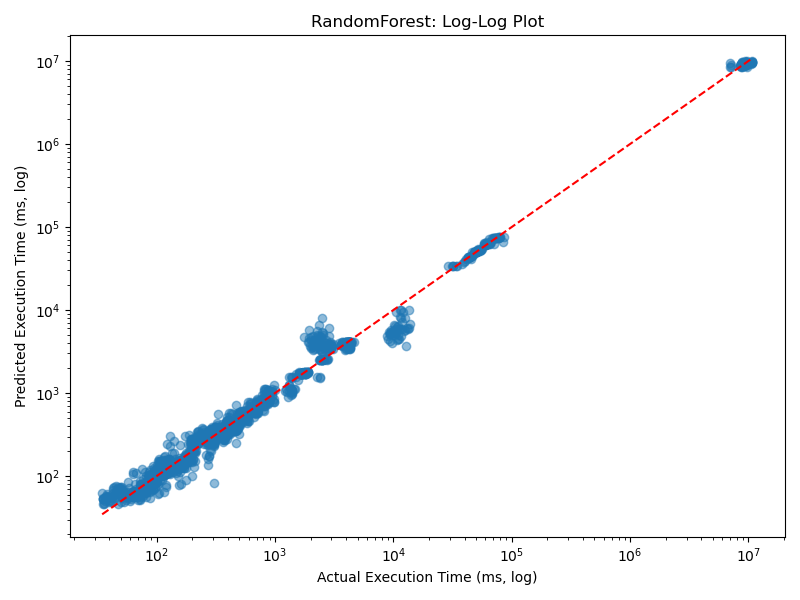
\includegraphics[width=\linewidth]{feature_based_rf/logscale.png}
  \caption{Random Forest Log-scale Predictions (Feature-Based)}
  \label{fig:rf-feature-log}
\end{figure}

\subsection{Regressions}
The first model that I made is a Feature-Based regression  to develop a predictive regression based on the following feature space:
\begin{multicols}{2}
\begin{itemize}
  \item Total Rows
  \item Total Loops
  \item Node Types
  \item Max Depth
  \item Has Seq Scan
  \item Has Sort
  \item Has Index Scan
  \item Workers Launched
  \item Query Id
\end{itemize}
\end{multicols}

For this feature space, I trained two regressions: a Random Forest regression and a XGBoost Regression. I performed hyperparameter tuning on both models to ensure that they achieved the best performance.
For performance statistics, I used Root Mean Square Error (RMSE), Mean Absolute Error (MAE), and R-squared metrics to determine their performance. It is also worth noting that for training purposes, I used the log
of the execution time, this is to make the variance more stable as there were outliers from Query 20 that were creating a very large imbalance in the data. We can see the results of the feature-based model in \ref{fig:rf-feature-log}
which shows a log-scaled plot of its Prediction vs. Actual Performance. I chose to log-scale these plots in order to better show the degree of variance that exists in the graph. As you can see there is a cluster of outliers that
are all from Query 20.


The second model that I implemented is a Query-based model. This model has a couple additional steps compared to the feature-based regression. Namely, I needed to encode the queries so that the regression could better
read and understand the text-based features. To do this I used sentence based transformers in order to encode this data \cite{reimers2019sentencebertsentenceembeddingsusing}. Once the data is encoded, I could then train the
regression. Similar to the feature-based, I used RMSE, MAE, and R-squared as the primary metrics. Figure \ref{fig:xgb-query-log} shows the XGBoost regression at log-scale and its performance.

\begin{figure}[h!]
  \centering
  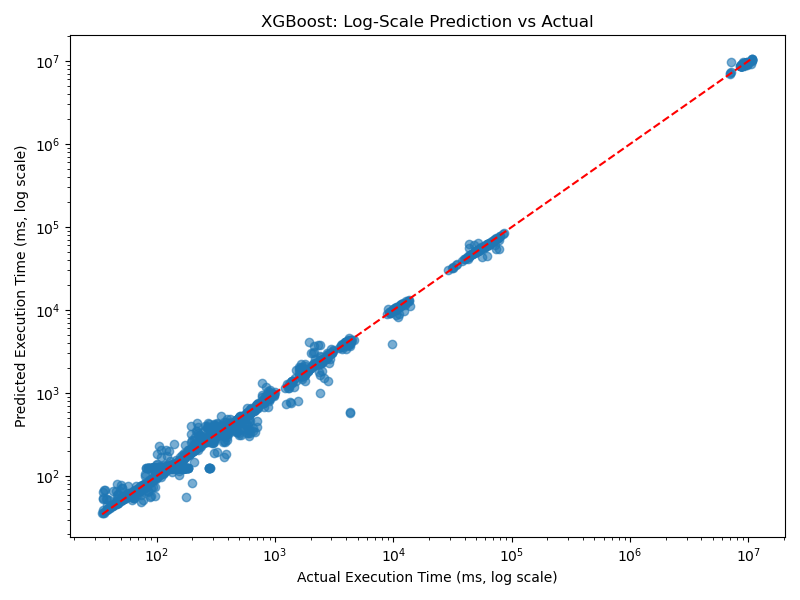
\includegraphics[width=\linewidth]{query_based_xgb/logscale.png}
  \caption{XGBoost Log-scale Predictions (Query-Based)}
  \label{fig:xgb-query-log}
\end{figure}

As we can see from Table \ref{tab:model-evaluation}, we can see that the query-based model outperformed the feature-based model.
This was actually quite a shocking revelation to me because of how much data the feature-based model was given. It is also worth it to note that while the RMSE and MAE are extremely high, that this is largely due to the outliers
that are present within Query 20 due to their unusually high execution times.

\begin{table}[h!]
  \centering
  \begin{tabular}{|l|l|r|r|r|}
    \hline
    \textbf{Model Type} & \textbf{Model}  & \textbf{RMSE (ms)} & \textbf{MAE (ms)} & \textbf{R\textsuperscript{2}} \\
    \hline
    \multirow{2}{*}{Feature-Based} 
      & RandomForest & 127,590.99 & 18,966.29 & 0.996 \\
      & XGBoost      & 143,512.72 & 22,809.43 & 0.995 \\
    \hline
    \multirow{2}{*}{Query-Based} 
      & RandomForest & 97,378.77 & 12,817.05 & 0.997 \\
      & XGBoost      & 77,019.35 & 8,337.39  & 0.998 \\
    \hline
  \end{tabular}
  \caption{Model evaluation results on full data (execution time in milliseconds)}
  \label{tab:model-evaluation}
\end{table}


\section{Challenges}
I ran into a few challenges with the execution of the tasks that I have completed thus far. Namely, I ran into issues with overly long executions and  Docker container setup.

\subsection{Long Query Execution}
For both the feature-based regression and the query-based regression, I needed to execute every query at least once. With 2200 queries in total, I knew that the execution would
take a long time; however, as I mentioned previously, Query 20 had some issues with large execution times. After a bit of further investigation it appears this is due to several nested
queries with various filters and joins which seem to be drastically increasing the execution times of this. In order to best overcome this issue, I attempted to optimize the query execution
script as much as possible. This involved parallelizing the process and increasing the number of CPU cores and the amount of RAM that the Docker container was allowed to access.
Even with all of this, it took on average over an hour for each query, and with 100 variations, this meant that it took over 3 days to run all of the executions. I also ran into a couple errors
with some of the executions which lead to a dataset less than the intended 1200.

\subsection{Docker Container Setup}
The setup of the Docker container was a little harder than I originally expected. I had to establish a bash script to run the SQL generator so that the database was populated upon the initial creation
of the container, and I also had to find the write similar commands to generate the 2200 queries that would be needed for execution. This was a lot of trial and error since it has been a while since I have
deployed my own container, but I figured it would be worth it in the event that this needed to be recreated or if I needed to scale the containers.

\section{Next Steps}
The next steps for the project will involve creating the genetic algorithm that will be used to create optimized queries. I hope to create a ``trainable'' algorithm that can then use the previously established
regressions to then predict its proposed query's execution, we can call this $t^*$. We can then compare $t^*$ to the actual execution time $t'$ to obtain an error that can then be used to train the algorithm further.
The idea being that this will produce a good optimizer using machine learning as a predictive backend to the optimizer. I do have some worries that I will run into challenges with figuring out the optimizer such that it
will work with the predictive model. I am still hopeful that I can get a genetic algorithm to work with this idea, but if it doesn't work, I might have to switch tactics.

\section{Conclusion}
Overall, I am very happy with the results that I have gotten from my two regression models. I am slightly annoyed with the Query 20 outliers, and I have considered multiple times as to whether I should get rid of Query 20
from the training and test cases entirely in order to make the Error and predictions seem more significant, but I think it is important to keep them in for representative purposes. I also think that the optimizer could potentially
improve the model to make it perform better as a whole.

\bibliographystyle{ACM-Reference-Format}
\bibliography{references}

\end{document}

